\subsection{Чистая архитектура} \label{clean-arch}
Clean Architecture - это популярный подход к разработке программного обеспечения, 
который был предложен Робертом Мартином (также известным как Uncle Bob). 
Этот подход помогает разработчикам создавать гибкие, расширяемые и легко тестируемые приложения.

В Golang Clean Architecture часто реализуется с помощью пакетов и интерфейсов. 
Пакеты используются для организации кода в логически связанные блоки, 
а интерфейсы - для определения контрактов между различными компонентами приложения.
На рисунке~\ref{clean-arch-pic} представлена схема такого взаимодействия пакетов.

\begin{figure}
    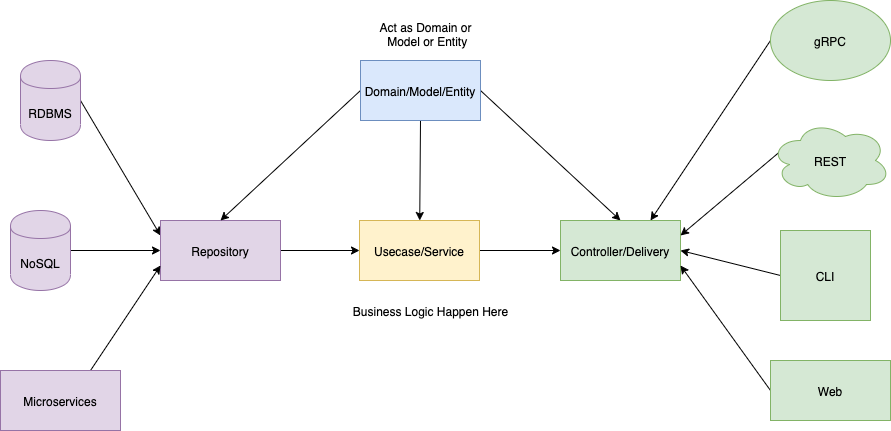
\includegraphics[scale=0.5]{imgs/clean-arch}
    \caption{Схема чистой архитектуры}
    \label{clean-arch-pic}
\end{figure}

В центре Clean Architecture находится принцип разделения зависимостей (Dependency Inversion Principle), который гласит, что зависимости должны быть направлены от абстракций к конкретным реализациям, а не наоборот.
Это позволяет разработчикам легко заменять реализации компонентов приложения, не затрагивая другие части системы.
Так, например, область, отвечающая за сохранение данных не должна содержать никакую логику.
Она должна только выдавать или сохранять данные.

Стоит оговориться, что не стоит обязательно точно придерживаться этому концепту.
Иногда в этом нет особой надобности.
Но такое разделение лучше делать всегда и сохранять его в том или ином виде.

Одним из основных преимуществ Clean Architecture в Golang является возможность легко тестировать каждый слой независимо от других. 
Это достигается путем использования интерфейсов для определения контрактов между слоями. 
Это позволяет разработчикам легко заменять реализации компонентов приложения на макеты (mocks) для тестирования.

Кроме того, Golang Clean Architecture обеспечивает высокую гибкость и расширяемость приложения. 
Благодаря разделению зависимостей и использованию интерфейсов, программисты могут легко добавлять новые функции и изменять существующие, не затрагивая другие части системы.

В Golang Clean Architecture используется многослойная архитектура.

\subsubsection{Представление (Presentation Layer)}
Этот слой отвечает за взаимодействие с пользователем и обработку входящих запросов.
Он содержит контроллеры, представления и другие компоненты, которые отображают данные для пользователя.
В вышеизложенном сервисе расположены хендлеры, которые отвечают за обработку запросов по конкретному роутингу.

\subsubsection{Использование (Use Case Layer)}
Этот слой содержит бизнес-логику приложения. 
Он определяет, как приложение должно взаимодействовать с данными и какие операции должны быть выполнены. 
Он также содержит интерфейсы для доступа к данным.
Например, в этом слое можно организовать логику парсинга картинок, организацию их по подгруппам и сбор в pdf.
Затем данные отправлять в следующий слой.

\subsubsection{Хранилище (Storage Layer)}
Этот слой отвечает за хранение данных и доступ к ним. 
Он содержит реализации интерфейсов, определенных в слое использования. 
Эти реализации могут использовать различные источники данных, такие как базы данных, файлы или внешние API.

\subsubsection{Инфраструктура (Infrastructure Layer)}
Этот слой содержит код, который не относится к бизнес-логике приложения, но необходим для его работы. 
Это может быть код для обработки ошибок, логирования, аутентификации и т.д. 
Этот слой также содержит реализации интерфейсов, определенных в слое использования, для доступа к внешним сервисам и системам.

На рисунке~\ref{clean-arch-add} демонстрируется пакетное представление проекта.